% ****************************************************************************************************
\chapter{Proof of Concept -- Using the Example of SAP HANA Cloud}\label{ch:poc}
% ****************************************************************************************************

In order to evaluate and show the applicability of the previous developed \ac{DSR} artifacts -- classification scheme (cf. Chapter \ref{ch:sota}), \ac{CLD} (cf. Chapter \ref{ch:cld}), and \ac{SFD} (cf. Chapter \ref{ch:sfd}) --, in the following a \acf{PoC} study using the example of the SAP HANA Cloud platform is presented. This approach is in conformity with the \ac{DSR} design cycle of \citet[pp. 88,90-91]{Hevner2007} and the \ac{DSR} activity evaluation according to \citet[p. 56]{Peffers2007}, whereby the artifacts have been evaluated against the real world by their reapplication in the context of \ac{PaaS} business models.

% ****************************************************************************************************
\section{Business Model Design Elements}\label{ch:poc:cs}
% ****************************************************************************************************

The business model of the SAP HANA Cloud platform is explained and illustrated, using the business model conceptualization proposed by \citet{Johnson2008}, in detail within Subsection \ref{ch:sota:sap}. In order to classify \ac{PaaS} business models, a corresponding classification scheme have been developed. How the SAP HANA Cloud platform addresses the identified classification criteria is briefly discussed below and illustrated in Figure \ref{fig:cs:sap} by means of a morphological box, whereas the addressed characteristics are highlighted.

Within the case study analysis of this platform, four diverse stakeholder groups, which are directly targeted, were identified -- application customer, development partners, platform customers, and individual developers. Using the classification scheme terminology, the SAP HANA Cloud platform addresses all five identified customer segments -- \ac{IT} startup, \ac{SI}, \ac{ISV}, platform customer, as well as application customer. However, these customer segments are served differently as illustrated further below. SAP HANA Cloud aims to support the development, deployment, and management of standalone as well as integrated cloud applications. However, the focus of this platform is rather to provide extensive integration features und thus classified as \ac{PaaS} platform with the core value proposition integration. The SAP HANA Cloud platform is neither an open source platform nor a highly regulated platform, hence a partly limited governance model is pursued. Meaning platform users of all characteristics have an extensive freedom of choice, although certain areas are regulated directly by the platform provider. Even though the SAP HANA Cloud platform is offering several technical capabilities, for instance the SAP Hana Cloud Eclipse plugin and corresponding \ac{SDK} (Java), they are considered rather as limited and thus for the criterion technical scope the characteristic limited technical capabilities is selected. In particular, the comparison with other \ac{PaaS} platforms and their technical capabilities support this classification. Based on the SAP HANA Cloud platform case study, three revenue streams which are used by this platform have been identified. First, platform customers are charged with subscription-based fees ranging from $370$ to $16.000$ \ac{EUR} monthly. Second, SAP takes a revenue share of $15\%$ for platform modules developed by complementors -- \acp{ISV} and \ac{IT} -- and distributed over the SAP store. Third, some charged addition services are offered, including annual development partner fees of $1.990$ \ac{EUR} and application certification fees ranging from $495$ to $990$ \ac{EUR}.

\begin{figure}[tb]
	\centering
	% ****************************************************************************************************
% Classification Scheme SAP
% ****************************************************************************************************

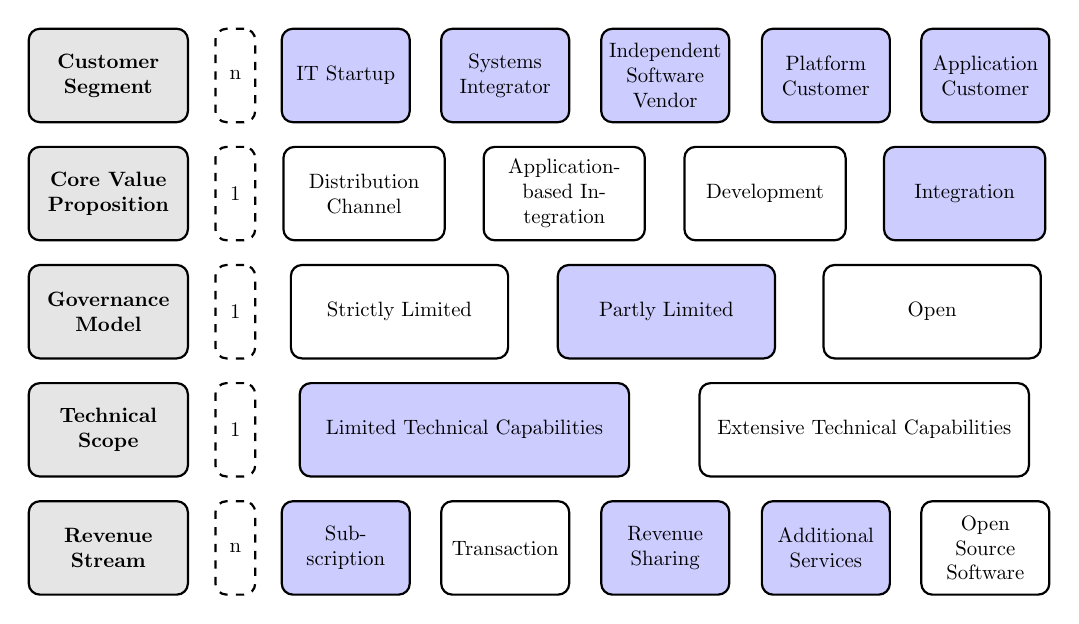
\begin{tikzpicture}[scale=0.75, every node/.style={scale=0.75}]

\node[font={\bfseries},draw,text width=7em,text centered,rectangle,rounded corners,minimum height=4.5em,thick,fill=gray!20] (1) at (-1,8) {Customer Segment};
\node[font={\bfseries},draw,text width=7em,text centered,rectangle,rounded corners,minimum height=4.5em,thick,fill=gray!20] (1) at (-1,6) {Core Value Proposition};
\node[font={\bfseries},draw,text width=7em,text centered,rectangle,rounded corners,minimum height=4.5em,thick,fill=gray!20] (1) at (-1,4) {Governance Model};
\node[font={\bfseries},draw,text width=7em,text centered,rectangle,rounded corners,minimum height=4.5em,thick,fill=gray!20] (1) at (-1,2) {Technical Scope};
\node[font={\bfseries},draw,text width=7em,text centered,rectangle,rounded corners,minimum height=4.5em,thick,fill=gray!20] (1) at (-1,0) {Revenue Stream};

\node[draw,text width=1.25em,text centered,rectangle,rounded corners,minimum height=4.5em,thick,dashed] (1) at (1.15,8) {n};
\node[draw,text width=1.25em,text centered,rectangle,rounded corners,minimum height=4.5em,thick,dashed] (1) at (1.15,6) {1};
\node[draw,text width=1.25em,text centered,rectangle,rounded corners,minimum height=4.5em,thick,dashed] (1) at (1.15,4) {1};
\node[draw,text width=1.25em,text centered,rectangle,rounded corners,minimum height=4.5em,thick,dashed] (1) at (1.15,2) {1};
\node[draw,text width=1.25em,text centered,rectangle,rounded corners,minimum height=4.5em,thick,dashed] (1) at (1.15,0) {n};

\node[draw,text width=5.5em,text centered,rectangle,rounded corners,minimum height=4.5em,thick,fill=blue!20] (1) at (3.02,8) {IT Startup};
\node[draw,text width=5.5em,text centered,rectangle,rounded corners,minimum height=4.5em,thick,fill=blue!20] (1) at (5.72,8) {Systems Integrator};
\node[draw,text width=5.5em,text centered,rectangle,rounded corners,minimum height=4.5em,thick,fill=blue!20] (1) at (8.43,8) {Independent Software Vendor};
\node[draw,text width=5.5em,text centered,rectangle,rounded corners,minimum height=4.5em,thick,fill=blue!20] (1) at (11.15,8) {Platform Customer};
\node[draw,text width=5.5em,text centered,rectangle,rounded corners,minimum height=4.5em,thick,fill=blue!20] (1) at (13.85,8) {Application Customer};

\node[draw,text width=7.1em,text centered,rectangle,rounded corners,minimum height=4.5em,thick] (1) at (3.33,6) {Distribution Channel};
\node[draw,text width=7.1em,text centered,rectangle,rounded corners,minimum height=4.5em,thick] (1) at (6.72,6) {Application-based Integration};
\node[draw,text width=7.1em,text centered,rectangle,rounded corners,minimum height=4.5em,thick] (1) at (10.12,6) {Development};
\node[draw,text width=7.1em,text centered,rectangle,rounded corners,minimum height=4.5em,thick,fill=blue!20] (1) at (13.5,6) {Integration};

\node[draw,text width=9.8em,text centered,rectangle,rounded corners,minimum height=4.5em,thick] (1) at (3.93,4) {Strictly Limited};
\node[draw,text width=9.8em,text centered,rectangle,rounded corners,minimum height=4.5em,thick,fill=blue!20] (1) at (8.45,4) {Partly Limited};
\node[draw,text width=9.8em,text centered,rectangle,rounded corners,minimum height=4.5em,thick] (1) at (12.95,4) {Open};

\node[draw,text width=15.2em,text centered,rectangle,rounded corners,minimum height=4.5em,thick,fill=blue!20] (1) at (5.03,2) {Limited Technical Capabilities};
\node[draw,text width=15.2em,text centered,rectangle,rounded corners,minimum height=4.5em,thick] (1) at (11.8,2) {Extensive Technical Capabilities};

\node[draw,text width=5.5em,text centered,rectangle,rounded corners,minimum height=4.5em,thick,fill=blue!20] (1) at (3.02,0) {Sub-scription};
\node[draw,text width=5.5em,text centered,rectangle,rounded corners,minimum height=4.5em,thick] (1) at (5.72,0) {Transaction};
\node[draw,text width=5.5em,text centered,rectangle,rounded corners,minimum height=4.5em,thick,fill=blue!20] (1) at (8.43,0) {Revenue Sharing};
\node[draw,text width=5.5em,text centered,rectangle,rounded corners,minimum height=4.5em,thick,fill=blue!20] (1) at (11.15,0) {Additional Services};
\node[draw,text width=5.5em,text centered,rectangle,rounded corners,minimum height=4.5em,thick] (1) at (13.85,0) {Open Source Software};

\end{tikzpicture}
	\caption{Proof of Concept -- Classification}
	\label{fig:cs:sap}
\end{figure}

As set out above, the classification scheme developed in this thesis can be easily used to initially assess and classify \ac{PaaS} business models and their characteristics. Whereby the classification schemewo is aimed to be as user friendly as possible -- a key classification guideline according to \citet[p. 41]{Fettke2003} -- and thereby ensuring that the classification criteria as well as their characteristics are comprehensible and sufficient.

% ****************************************************************************************************
\section{Qualitative Findings}\label{ch:poc:qf}
% ****************************************************************************************************

Based on the previous developed \acp{CLD} (cf. Figures \ref{fig:cld_cs} - \ref{fig:cld_bp}) \ac{PaaS} business models and their inherent dynamics can be investigated and lead finally to a better understanding of their impacts.

As illustrated in Figure \ref{fig:cld_cs}, six basic factors influencing the \acp{CVP} for all customer segments have been discussed. First, the core value proposition of the SAP HANA Cloud platform which has a direct impact on the \acp{CVP} is, as mentioned above, integration-focused. This focus seems appropriate for all five customer segments: complementors -- \acp{ISV} and \ac{IT} startups -- developing integration-based platform modules, platform customers developing internal integration solutions, application customers using platform modules for integration purposes, and \acp{SI} providing corresponding consultancy services. Second, the partly limited governance model might also positively influence the \acp{CVP} for \acp{ISV}, \ac{IT} startups, and platform customers, although this might not have much influence on \acp{SI} and application customers. Third, the rather limited technical scope (limited technical capabilities) will, in the best case, not strengthen the \acp{CVP} especially for \acp{ISV}, \ac{IT} startups, and platform customers. However, in the worst case this limited technical scope will change to the contrary and negatively influence the \acp{CVP}. Fourth, although some additional services are offered and thus positively influence the \acp{CVP} particularly for \acp{ISV} and \ac{IT} startups, a broader range of additional services dedicated to all targeted customer segments would increase this impact lasting. Fifth, as discussed in Section \ref {ch:cld:cs} and in line with \citet[p. 200]{Evans2003} platform improvements lead to improved \acp{CVP}, but also enlarge the technical scope and wider the range of additional services. Due to the fact the quantities revenue and improvements, which result in platform improvements, are unknown, the actual impact of the self-reinforcing feedback loops R\_2, R\_3, and R\_4 associated with platform improvements (cf. Figure \ref{fig:cld_cs}) are rather cloudy. Sixth, the overall market penetration of the SAP HANA Cloud platform is currently rather low and influences the \acp{CVP} scarcely perceptible. This impact might change with an increase in the customer base leading to an increased overall market penetration as indicated by the self-reinforcing feedback loop R\_5 in Figure \ref{fig:cld_cs}.

Using the generic \ac{PaaS} customer segment \ac{CLD}, \ac{PaaS} business models can be analyzed with regard to the adoption dynamics and first conclusions can be drawn. In case of the SAP HANA Cloud platform the most significant remark so far concerns the technical scope. By individual consideration and even more in comparison with other \ac{PaaS} platforms offering the core value proposition integration, the currently offered technical capabilities are not sufficient. Hence, enlarging the technical scope might lead to substantial \ac{CVP} enhancements.

The inherent and crucial cross-sided network effects between the five \ac{PaaS} customer segments have been discussed in Section \ref{ch:cld:csi} and illustrated by means of a \ac{CLD} (cf. Figure \ref{fig:cld_csi}). Since the SAP HANA Cloud platform is addressing all five customer segments, this \ac{CLD} cannot be simplified, nevertheless valuable insights can be gained.

Platform modules have been identified to influence -- directly and indirectly -- all customer segments. These platform complements are developed and provided by complementors -- \acp{ISV} and \ac{IT} startups -- and are valuable mainly for platform and application customers but also for \acp{SI}. However, only a few ready to use applications built upon the SAP HANA Cloud platform, which might be used by application customers, are offered at present. Hence, the self-reinforcing feedback loops R\_8 and R\_9 (cf. Figure \ref{fig:cld_csi}) will only have weak impacts. Since just a few applications (platform modules) are available, the \ac{CVP} for application customers will remain weak and consequently the application customer population will not increase considerable. This implies that due to the few application customers the \acp{CVP} for \acp{ISV} and \ac{IT} startups are not significant improved and thus the number of platform modules stays constant. Furthermore, in order to sell platform modules built upon the SAP HANA Cloud platform via the SAP Store, the so called development partners -- \acp{ISV} and \ac{IT} startups -- are charged literally just to be such a development partner ($1.990$ \ac{EUR} yearly) and in addition these applications need go through a charged certification process (initial $990$ \ac{EUR} and yearly recurring $495$ \ac{EUR}). All these facts and circumstances taken together lead to the unpleasant, but not unusual, situation in which platform providers face in their early stages the chicken and egg launch problem. Since this problem is not unfamiliar, approaches so as to overcome this problem are present. For instance, a typical approach to solve this problem is subsidizing one or more customer segments through incentives as discussed by \citet[pp. 1,5]{Eisenmann2006} and \citet[pp. 195-196]{Evans2003}. Platform customers on the other hand are also influenced through platform modules, although less strongly because they utilize platform modules in addition to the actually used platform and not solely as the customer segment application customers. Consequently, also the feedback loops R\_10 and R\_11 (cf. Figure \ref{fig:cld_csi}) connecting the variables platform customers and platform modules remain rather weak due to the manageable number of platform modules. Finally, since the variables platform and application customers as well as platform modules are relatively low, the \ac{CVP} for \acp{SI} is not influenced positively through these factors. As a result the two self-reinforcing feedback loops R\_6 and R\_7 (cf. Figure \ref{fig:cld_csi}) are almost immaterial.

The application of the developed \ac{CLD} artifact (cf. Figure \ref{fig:cld_bp}) in the real world scenario of the SAP HANA Cloud platform clearly identifies two emphases, where SAP might improve their business model. First, as mentioned above the currently offered technical capabilities are not sufficient and prevent the platform to establish oneself. Extending the technical scope might particularly increase the \acp{CVP} for \acp{ISV}, \ac{IT} startups, and platform customers. Second, so far the SAP HANA Cloud platform does not create significant cross-sided network effects which have been identified to be essential in the platform adoption process. Instead of experiencing a flourishing platform and its network effects, the common chicken and egg launch problem is faced. SAP might work on these cross-sided network effects and try to create and capture more of them in order to overcome this obstacle, for instance by subsidizing quality- or price-sensitive customers.

% ****************************************************************************************************
\section{Simulation Results}\label{ch:poc:sr}
% ****************************************************************************************************

% zwei modellierungsarten: abolut und relative


\begin{table}[t]
	\centering
	\begin{tabular}{llllllll}
		\toprule 
		\multicolumn{8}{c}{\footnotesize \textbf{Variables and their corresponding Values}} \\ \midrule
		\footnotesize $GOV(t_0)$ & \footnotesize $0.6$ & \footnotesize $CVP_{ITS}(t_0)$ & \footnotesize $0.04$ & \footnotesize $P_{IN_{ITS}}$ & \footnotesize $0.005$ & \footnotesize $P_{IM_{ITS}}$ & \footnotesize $0.01$ \\
		\footnotesize $TS(t_0)$ & \footnotesize $0.5$ & \footnotesize $CVP_{SI}(t_0)$ & \footnotesize $0.03$ & \footnotesize $P_{IN_{SI}}$ & \footnotesize $0.0125$ & \footnotesize $P_{IM_{SI}}$ & \footnotesize $0.025$ \\
		\footnotesize $AS(t_0)$ & \footnotesize $0.4$ & \footnotesize $CVP_{ISV}(t_0)$ & \footnotesize $0.05$ & \footnotesize $P_{IN_{ISV}}$ & \footnotesize $0.005$ & \footnotesize $P_{IM_{ISV}}$ & \footnotesize $0.01$ \\
		& & \footnotesize $CVP_{PC}(t_0)$ & \footnotesize $0.07$ & \footnotesize $P_{IN_{PC}}$ & \footnotesize $0.0125$ & \footnotesize $P_{IM_{PC}}$ & \footnotesize $0.025$ \\
		& & \footnotesize $CVP_{AC}(t_0)$ & \footnotesize $0.01$ & \footnotesize $P_{IN_{AC}}$ & \footnotesize $0.01$ & \footnotesize $P_{IM_{AC}}$ & \footnotesize $0.02$ \\ \bottomrule
	\end{tabular}
	\caption{Proof of Concept -- Simulation Variables}
	\label{tab:mvar:sap}
\end{table}




\begin{figure}[htb]
	\centering
	% ****************************************************************************************************
% Graph Population Customer Segments Stocks
% ****************************************************************************************************

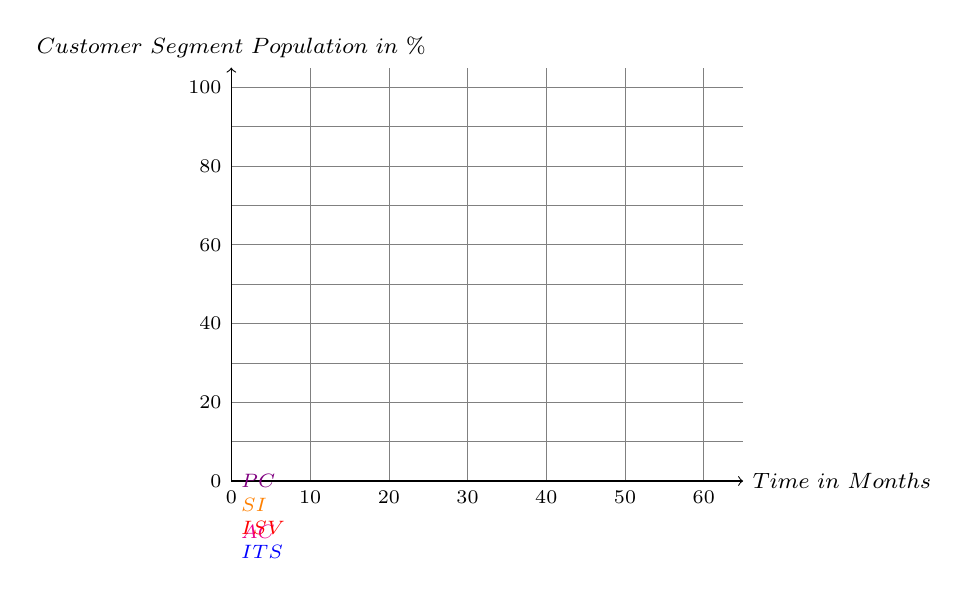
\begin{tikzpicture}[x=0.1cm,y=0.05cm]

  \def\xmin{0}
  \def\xmax{65}
  \def\ymin{0}
  \def\ymax{105}

  % grid
  \draw[style=help lines, ystep=10, xstep=10] (\xmin,\ymin) grid
  (\xmax,\ymax);

  % axes
  \draw[->] (\xmin,\ymin) -- (\xmax,\ymin) node[right] {\footnotesize $Time~in~Months$};
  \draw[->] (\xmin,\ymin) -- (\xmin,\ymax) node[above] {\footnotesize $Customer~Segment~Population~in~\%$};

  \foreach \x in {0,10,...,60}
    \node at (\x, \ymin) [below] {\scriptsize \x};
  \foreach \y in {0,20,...,100}
    \node at (\xmin,\y) [left] {\scriptsize \y};

  %,mark=*,mark size=0.5pt
	\draw[color=magenta] plot[smooth] file {simulationData/AC/populationAC.txt}
			node [below=0.65cm,right] {\scriptsize $AC$};
	\draw[color=blue] plot[smooth] file {simulationData/ITS/populationITS.txt}
			node [below=0.9cm,right] {\scriptsize $ITS$};	
	\draw[color=red] plot[smooth] file {simulationData/ISV/populationISV.txt}
			node [below=0.6cm,right] {\scriptsize $ISV$};	
	\draw[color=orange] plot[smooth] file {simulationData/SI/populationSI.txt}
			node [below=0.3cm,right] {\scriptsize $SI$};	
	\draw[color=violet] plot[smooth] file {simulationData/PC/populationPC.txt}
			node [right] {\scriptsize $PC$};	
												
\end{tikzpicture}

	\caption{Proof of Concept Simulation -- Customers}
\end{figure}

\begin{figure}[htb]
	\centering
	% ****************************************************************************************************
% Graph Potential Customer Segments Stocks
% ****************************************************************************************************

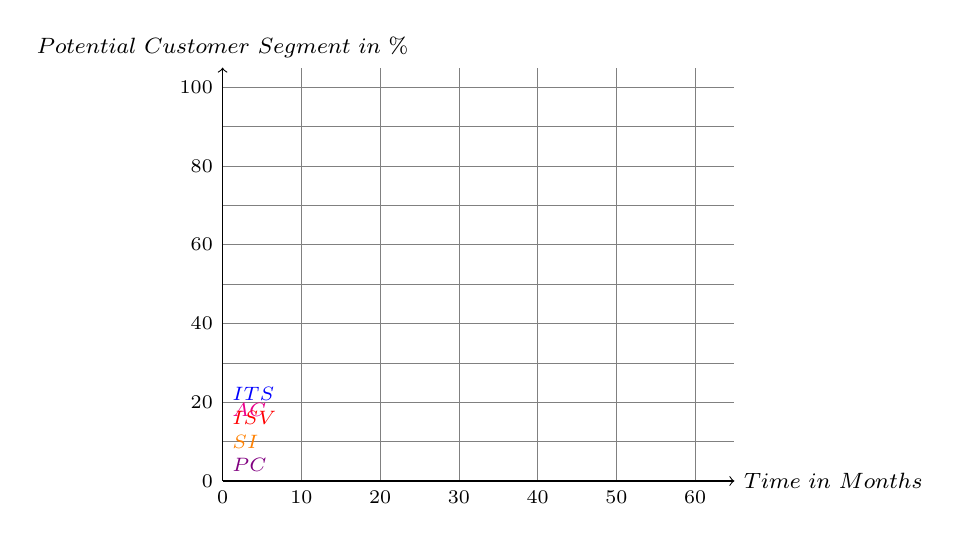
\begin{tikzpicture}[x=0.1cm,y=0.05cm]

  \def\xmin{0}
  \def\xmax{65}
  \def\ymin{0}
  \def\ymax{105}

  % grid
  \draw[style=help lines, ystep=10, xstep=10] (\xmin,\ymin) grid
  (\xmax,\ymax);

  % axes
  \draw[->] (\xmin,\ymin) -- (\xmax,\ymin) node[right] {\footnotesize $Time~in~Months$};
  \draw[->] (\xmin,\ymin) -- (\xmin,\ymax) node[above] {\footnotesize $Potential~Customer~Segment~in~\%$};

  \foreach \x in {0,10,...,60}
    \node at (\x, \ymin) [below] {\scriptsize \x};
  \foreach \y in {0,20,...,100}
    \node at (\xmin,\y) [left] {\scriptsize \y};

  %,mark=*,mark size=0.5pt
	\draw[color=magenta] plot[smooth] file {simulationData/AC/potentialAC.txt}
			node [above=0.9cm,right] {\scriptsize $AC$};
	\draw[color=blue] plot[smooth] file {simulationData/ITS/potentialITS.txt}
			node [above=1.1cm,right] {\scriptsize $ITS$};	
	\draw[color=red] plot[smooth] file {simulationData/ISV/potentialISV.txt}
			node [above=0.8cm,right] {\scriptsize $ISV$};	
	\draw[color=orange] plot[smooth] file {simulationData/SI/potentialSI.txt}
			node [above=0.5cm,right] {\scriptsize $SI$};	
	\draw[color=violet] plot[smooth] file {simulationData/PC/potentialPC.txt}
			node [above=0.2cm,right] {\scriptsize $PC$};	
	
													
\end{tikzpicture}

	\caption{Proof of Concept Simulation -- Potential Customers}
\end{figure}

\begin{figure}[htb]
	\centering
	% ****************************************************************************************************
% Graph Overall Adoption 
% ****************************************************************************************************

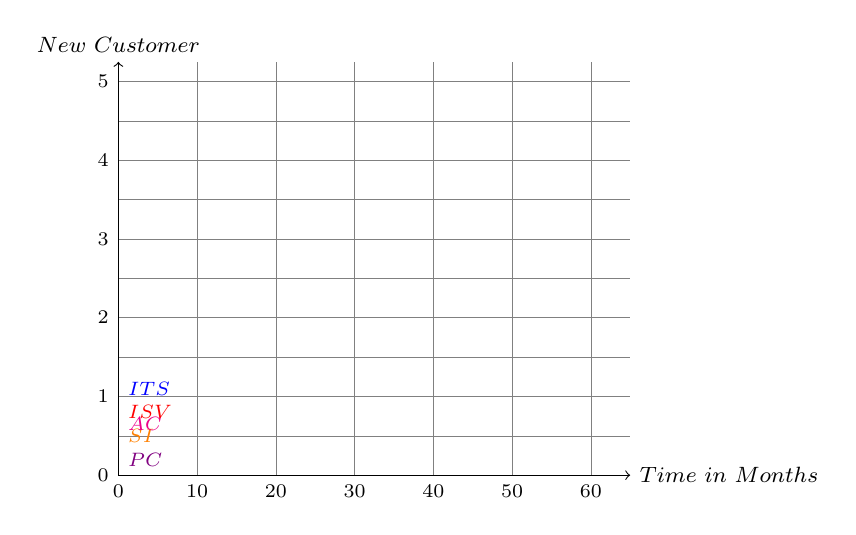
\begin{tikzpicture}[x=0.1cm,y=1cm]

  \def\xmin{0}
  \def\xmax{65}
  \def\ymin{0}
  \def\ymax{5.25}

  % grid
  \draw[style=help lines, ystep=0.5, xstep=10] (\xmin,\ymin) grid
  (\xmax,\ymax);

  % axes
  \draw[->] (\xmin,\ymin) -- (\xmax,\ymin) node[right] {\footnotesize $Time~in~Months$};
  \draw[->] (\xmin,\ymin) -- (\xmin,\ymax) node[above] {\footnotesize $New~Customer$};

  \foreach \x in {0,10,...,60}
    \node at (\x, \ymin) [below] {\scriptsize \x};
  \foreach \y in {0,1,...,5}
    \node at (\xmin,\y) [left] {\scriptsize \y};

  %,mark=*,mark size=0.5pt
	\draw[color=orange] plot[smooth] file {simulationData/SI/adoptionSI.txt}
			node [above=0.5cm, right] {\scriptsize $SI$};
	\draw[color=violet] plot[smooth] file {simulationData/PC/adoptionPC.txt}
			node [above=0.2cm, right] {\scriptsize $PC$};
	\draw[color=magenta] plot[smooth] file {simulationData/AC/adoptionAC.txt}
			node [above=0.65cm, right] {\scriptsize $AC$};
	\draw[color=red] plot[smooth] file {simulationData/ISV/adoptionISV.txt}
			node [above=0.8cm, right] {\scriptsize $ISV$};
	\draw[color=blue] plot[smooth] file {simulationData/ITS/adoptionITS.txt}
			node [above=1.1cm, right] {\scriptsize $ITS$};										
		
\end{tikzpicture}

	\caption{Proof of Concept Simulation -- New Customers}
\end{figure}


